% Instructions to change to html version:
% Comment out:
%  minipage, multicols,columnbreak, mathbf, hrule
% Replace all: \begin{minipage}% \end{minipage} %\begin{mulicols}  %\end{mulicols}  %\columnbreak % \begin{framed} %\end{framed} %\hrule
% Search for \mathbf
% Replace \)\) with \[ and $ with \(
% Enclose graphics in figure environments and add captions
% Re-tag \df environments as sections, subsections, etc.
% Command Line Code to Create html version:
%First: pdflatex -shell-escape filename.tex                                   
%Second, for each figure: inkscape "filename-figure1.pdf" -o "filename-figure1.png"
% Third: htlatex filename.tex "ht5mjlatex.cfg, charset=utf-8" " -cunihtf -utf8"
\documentclass[10pt]{article}

%\usepackage{tikz, pgf,pgfplots,wasysym,array}
%\usepackage{wasysym,array}

\usepackage{amsmath,amssymb}

\ifdefined\HCode
  \def\pgfsysdriver{pgfsys-tex4ht-updated.def}
\fi 
%\ifdefined\HCode
%  \def\pgfsysdriver{pgfsys-dvisvgm4ht.def}
%\fi 
\usepackage{tikz}
\usetikzlibrary{calc,decorations.markings,arrows}
\usepackage{pgfplots}

\pgfplotsset{compat=1.12}
\usepackage{myexternalize}
\usetikzlibrary{calc,decorations.markings,arrows}
\usepackage{framed}
\usepackage[none]{hyphenat}

\input{../../../common/1336_header_test.tex}
% \input{header.tex}

\usepackage{multirow, array}
\begin{document}

\everymath{\displaystyle}

\renewcommand{\myTitle}{MATH 1336: Calculus III}

\renewcommand{\mySubTitle}{Section 1.2: Calculus with Parametric Curves, Part 2}
%~\hfill Name: \underline{~~~~~~~~~~~~~~~~~~~~~~~~~~~~~~~~~~~~~~~~~~~~~~~}

\lectTitle{\vspace*{-.5in}\myTitle}{\vspace*{.1in}\mySubTitle \vspace*{-.25in}}


\setlength{\columnseprule}{0.4pt}
\setlength{\columnsep}{3em}

%\hspace*{-.8in}\begin{minipage}{1.25\textwidth}
%\begin{framed}

\section*{Integral Calculus with Parametric Curves:}
Consider a curve \(C\) on the interval \(a\leq x \leq b\) with parametric equations
\[
x = x(t), \quad y = y(t), \quad \alpha \leq t \leq \beta
\]

We would like to extend the concepts of \textbf{area} and \textbf{arclength} from Integral Calculus to the new setting of parametric curves.\\

%\vspace*{.1in}
%\hrule
%\vspace*{.1in}

%\begin{minipage}{.4\textwidth}

\begin{figure}[!h]

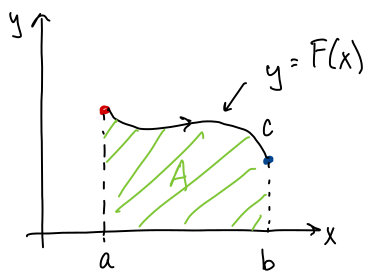
\includegraphics[width=\textwidth]{parametric-area.png}
\caption{Diagram illustrating finding the area under a parametric curve.}

\end{figure}

%\end{minipage}
\hspace*{.2in}
%\begin{minipage}{.5\textwidth}

%\underline{\textbf{\Large Potentially Useful Formulas:}}\\~\\
%\small
\textbf{Area:}\\
To calculate the area under the curve \(y = F(x)\) from \(x=a\) to \(x=b\):

\[
A = \int_a^b F(x)\ dx  = \int_a^b y\ dx  = \int_\alpha^\beta y(t)\ x'(t)\ dt%, \qquad A = \int_\alpha^\beta \frac{1}{2}r^2 \ d\theta
\]

The set-up above is for a curve that is parametrized from left to right: 
\[a = x(\alpha),\ b = x(\beta).\]

If the curve is parametrized from right to left, the limits of integration should be swapped so that the lower limit of integration corresponds to the left endpoint of the interval, \(x=a\), and the upper limit of integration corresponds to the right endpoint of the interval, \(x=b\).

%\end{minipage}

%\vspace*{.1in}
%\hrule
%\vspace*{.1in}

%\begin{minipage}{.4\textwidth}

\begin{figure}[!h]

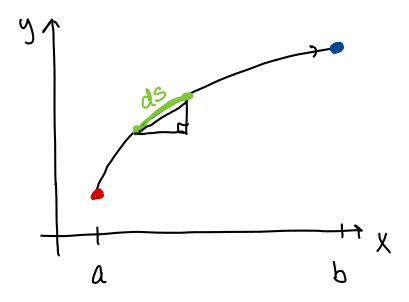
\includegraphics[width=\textwidth]{parametric-arclength.png}
\caption{Diagram illustrating finding the length of a parametric curve.}
\end{figure}

%\end{minipage}
\hspace*{.2in}
%\begin{minipage}{.5\textwidth}

\textbf{Arclength:}\\
To calculate the length, \(L\), of the parametric curve from \(t=\alpha\) to \(t = \beta\), set up the following integral, where \(ds\) is the infinitesimal distance element along the curve:

\[
L= \int ds = \int_{\alpha}^{\beta} \sqrt{\left(\frac{dx}{dt}\right)^2 + \left(\frac{dy}{dt}\right)^2}\ dt %\qquad L= \int_{\alpha}^{\beta} \sqrt{r^2 + \left(\frac{dr}{d\theta}\right)^2}\ d\theta
\]

Note that the expression for \(ds\) comes from the Pythagorean theorem, and the idea that in the limit as each of the distance elements go to zero:
\[
\left(\frac{ds}{dt}\right)^2 = \left(\frac{dx}{dt}\right)^2 + \left(\frac{dy}{dt}\right)^2
\]
%
%\vspace*{-.2in}
%\end{minipage}

%\end{framed}
%\end{minipage}

%\pagebreak

%\vspace*{-.5in}
\section*{In-Class Problems:}

We will work through Problem 1 together, then work on the remaining problems in small groups.

\vfill

%\begin{flushright}
%\textit{(See next page)}
%\end{flushright}
%
%\pagebreak

\begin{enumerate}%[{Problem} 1:]

\item Consider the curve described by the following parametric equations, which is graphed on the axes below.
\[
x=1+3t^2, \qquad y = 4+2t^3, \qquad 0\leq t\leq 1
\]
%\begin{multicols}{2}
%\begin{minipage}{.4\textwidth}
%\hspace*{-.5in}
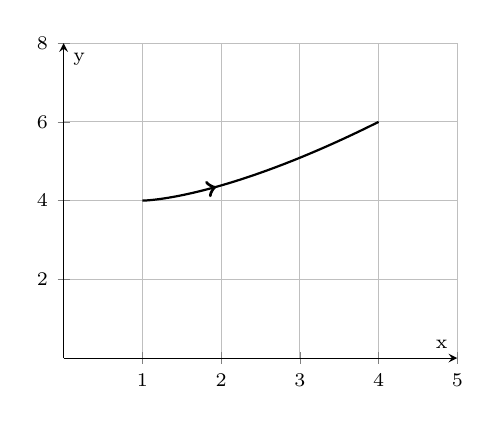
\begin{tikzpicture}
\begin{axis}[
	y=.5cm,
    x=1cm,
	axis x line=middle,
	axis y line = middle,
	ymin=0,ymax=8,
%	xmin=-.1,xmax=6,
	xmin=0,xmax=5,
    grid=both,
%    ticks=none,
%    yticklabels={},
%    xticklabels={},
    %xtick={0,1,...,6},
    xtick={0,1,...,5},
    ytick={0,2,...,8},
    xlabel=x,
    ylabel=y,
    label style={font=\scriptsize},
    tick label style={font=\scriptsize}
]




%\addplot[thick,black,variable=\t, domain=-3:3,samples=100,decoration = {markings,
%    mark = at position .3 with {\arrow[line width=1.2pt]{>}}
%  }, postaction = decorate] ({t^2}, {(t^3)/3 - t});
  \addplot[thick,black,variable=\t, domain=-0:1,samples=200,decoration = {markings,
    mark = at position .3 with {\arrow[line width=1.2pt]{>}}
  }, postaction = decorate] ({1+3*t^2}, {4+2*t^3});
%\addplot+[black,only marks, mark=*, line width=2pt] coordinates{(5,0)(0,5)};
%\node [above] at (axis cs:  .15,.25) {\(C\)};

\end{axis}
%\filldraw[fill=green!20,draw=green!50!black] (1.5cm,0cm) -- (3.75cm,0cm) arc
%(0:45:3.75cm) -- (1.065cm,1.065cm) arc (45:0:1.5cm) -- cycle;
%
%

\end{tikzpicture}
%\end{minipage}

%\columnbreak
\begin{enumerate}
\item Set up and evaluate a definite integral to calculate the area under the curve between \(t=0\) and \(t=1\).
\item Does your answer seem reasonable? Explain why or why not.
\item Set up and evaluate a definite integral to calculate the length of the curve between \(t=0\) and \(t=1\).
\item Does your answer seem reasonable? Explain why or why not.
\end{enumerate}

%\end{multicols}

\vfill

%\vspace*{-2in}
%\pagebreak

\item Consider the curve described by the following parametric equations, which is graphed on the axes below.
\[
x=e^t, \qquad y =5-2t, \qquad 0\leq t\leq 3
\]
%\begin{multicols}{2}
%\begin{minipage}{.4\textwidth}
%\hspace*{-.5in}
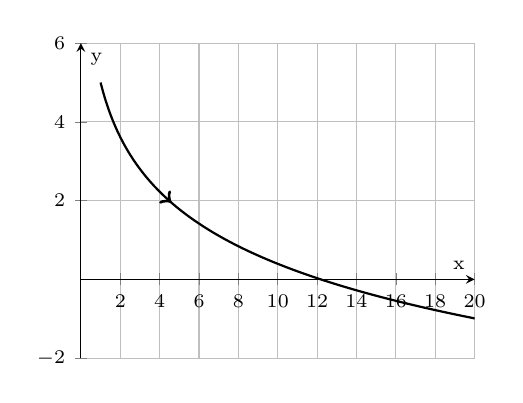
\begin{tikzpicture}
\begin{axis}[
	y=.5cm,
    x=.25cm,
	axis x line=middle,
	axis y line = middle,
	ymin=-2,ymax=6,
%	xmin=-.1,xmax=6,
	xmin=0,xmax=20,
    grid=both,
%    ticks=none,
%    yticklabels={},
%    xticklabels={},
    %xtick={0,1,...,6},
    xtick={0,2,...,20},
    ytick={-2,0,...,6},
    xlabel=x,
    ylabel=y,
    label style={font=\scriptsize},
    tick label style={font=\scriptsize}
]




%\addplot[thick,black,variable=\t, domain=-3:3,samples=100,decoration = {markings,
%    mark = at position .3 with {\arrow[line width=1.2pt]{>}}
%  }, postaction = decorate] ({t^2}, {(t^3)/3 - t});
  \addplot[thick,black,variable=\t, domain=0:3,samples=200,decoration = {markings,
    mark = at position .3 with {\arrow[line width=1.2pt]{>}}
  }, postaction = decorate] ({e^t}, {5-2*t});
%\addplot+[black,only marks, mark=*, line width=2pt] coordinates{(5,0)(0,5)};
%\node [above] at (axis cs:  .15,.25) {\(C\)};

\end{axis}
%\filldraw[fill=green!20,draw=green!50!black] (1.5cm,0cm) -- (3.75cm,0cm) arc
%(0:45:3.75cm) -- (1.065cm,1.065cm) arc (45:0:1.5cm) -- cycle;
%
%

\end{tikzpicture}
%\end{minipage}

%\columnbreak
\begin{enumerate}
\item Set up and evaluate a definite integral to calculate the area under the curve between \(t=0\) and \(t=3\).
\item Does your answer seem reasonable? Explain why or why not.
\item Set up, but \textbf{DO NOT} evaluate, a definite integral to calculate the length of the curve between \(t=0\) and \(t=3\).
\end{enumerate}

%\end{multicols}


%\pagebreak

\vfill
\item Consider the \textbf{Astroid} described by the following parametric equations, which is graphed on the axes below.
\[
x=\cos^3(t), \qquad y =\sin^3(t), \qquad 0\leq t\leq 2\pi
\]
%\begin{multicols}{2}
%\begin{minipage}{.4\textwidth}
%\hspace*{-.5in}
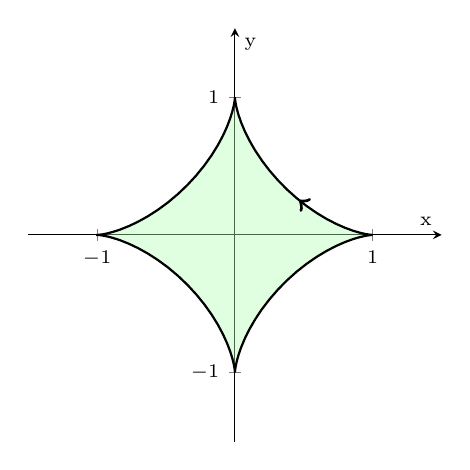
\begin{tikzpicture}
\begin{axis}[
	y=1.75cm,
    x=1.75cm,
	axis x line=middle,
	axis y line = middle,
	ymin=-1.5,ymax=1.5,
	xmin=-1.5,xmax=1.5,
    grid=none,
%    ticks=none,
%    yticklabels={},
%    xticklabels={},
    xtick={-1,0,...,1},
    ytick={-1,0,...,1},
    xlabel=x,
    ylabel=y,
    label style={font=\scriptsize},
    tick label style={font=\scriptsize}
]




\addplot[thick,black,variable=\t, domain=0:2*pi,samples=100,fill=green!30, fill opacity=.4, decoration = {markings,
    mark = at position .1 with {\arrow[line width=1.2pt]{>}}
  }, postaction = decorate] ({cos(deg(t))^3},{sin(deg(t))^3});
%\addplot+[black,only marks, mark=*, line width=2pt] coordinates{(5,0)(0,5)};
%\node [above] at (axis cs:  .15,.25) {\(C\)};


\end{axis}
%\filldraw[fill=green!20,draw=green!50!black] (1.5cm,0cm) -- (3.75cm,0cm) arc
%(0:45:3.75cm) -- (1.065cm,1.065cm) arc (45:0:1.5cm) -- cycle;
%
%

\end{tikzpicture}
%\end{minipage}

%\columnbreak
\begin{enumerate}
\item Find the coordinates of the points corresponding to \(t=0\) and \(t=\pi/2\).
\item Set up and evaluate a definite integral to calculate \(L_1\): the length of the part of the curve that lies in the first quadrant.
\item Use the value that you calculated for \(L_1\) to calculate the length of the entire Astroid.
\item Does your answer seem reasonable? Explain why or why not.
\item Set up, but \textbf{DO NOT} evaluate, a definite integral to calculate \(A_1\): the area under the part of the curve that lies in the first quadrant.
\end{enumerate}

%\end{multicols}


\end{enumerate}


\end{document}
